%!TEX root = ../physical-olympics-2.tex
\chapter{刚体}


\section{刚体的物理描述}
近代以前人们意识到了物质世界的\emph{连续性}(continuum),\,同时针锋相对地也提出了\emph{原子论}(atomism).\,原子最简单的模型就是质点,\,而调和物质连续性与原子学说的中间模型就是\emph{刚体}(rigid body)模型.\,刚体是不允许形变发生的系统.\,由牛顿力学对质点的讨论推广到质点系的讨论,\,使我们也很容易将相关结论进一步推广到刚体.

由于刚体上一点受力,\,则整体同时运动起来,\,这个模型与相对论力学体系是不兼容的.\,具体来说,\,相互作用必须以有限的速度传播,\,否则就违背了因果律.\,刚体不符合因果律这一时空的固有结构.\,在很多相对论情境下将招致矛盾的结果.

刚体的物理学量是哪一些呢?\,必要的内禀的属性是其质量的分布.\,某一默认时刻$t_0$刚体占据了空间区域$\Omega_0$,\,由大量体积微元$\ud V$(记做$\ud^3\bs{R}_0$)组成,\,则刚体的总质量为:
\[m=\int\limits_{\Omega_0}\rho(\bs{R}_0)\ud^3\bs{R}_0=\int\limits_{\Omega_0}\ud m\]

\begin{wrapfigure}[17]{o}[-10pt]{7cm}
\vspace{-0.4cm}
\centering
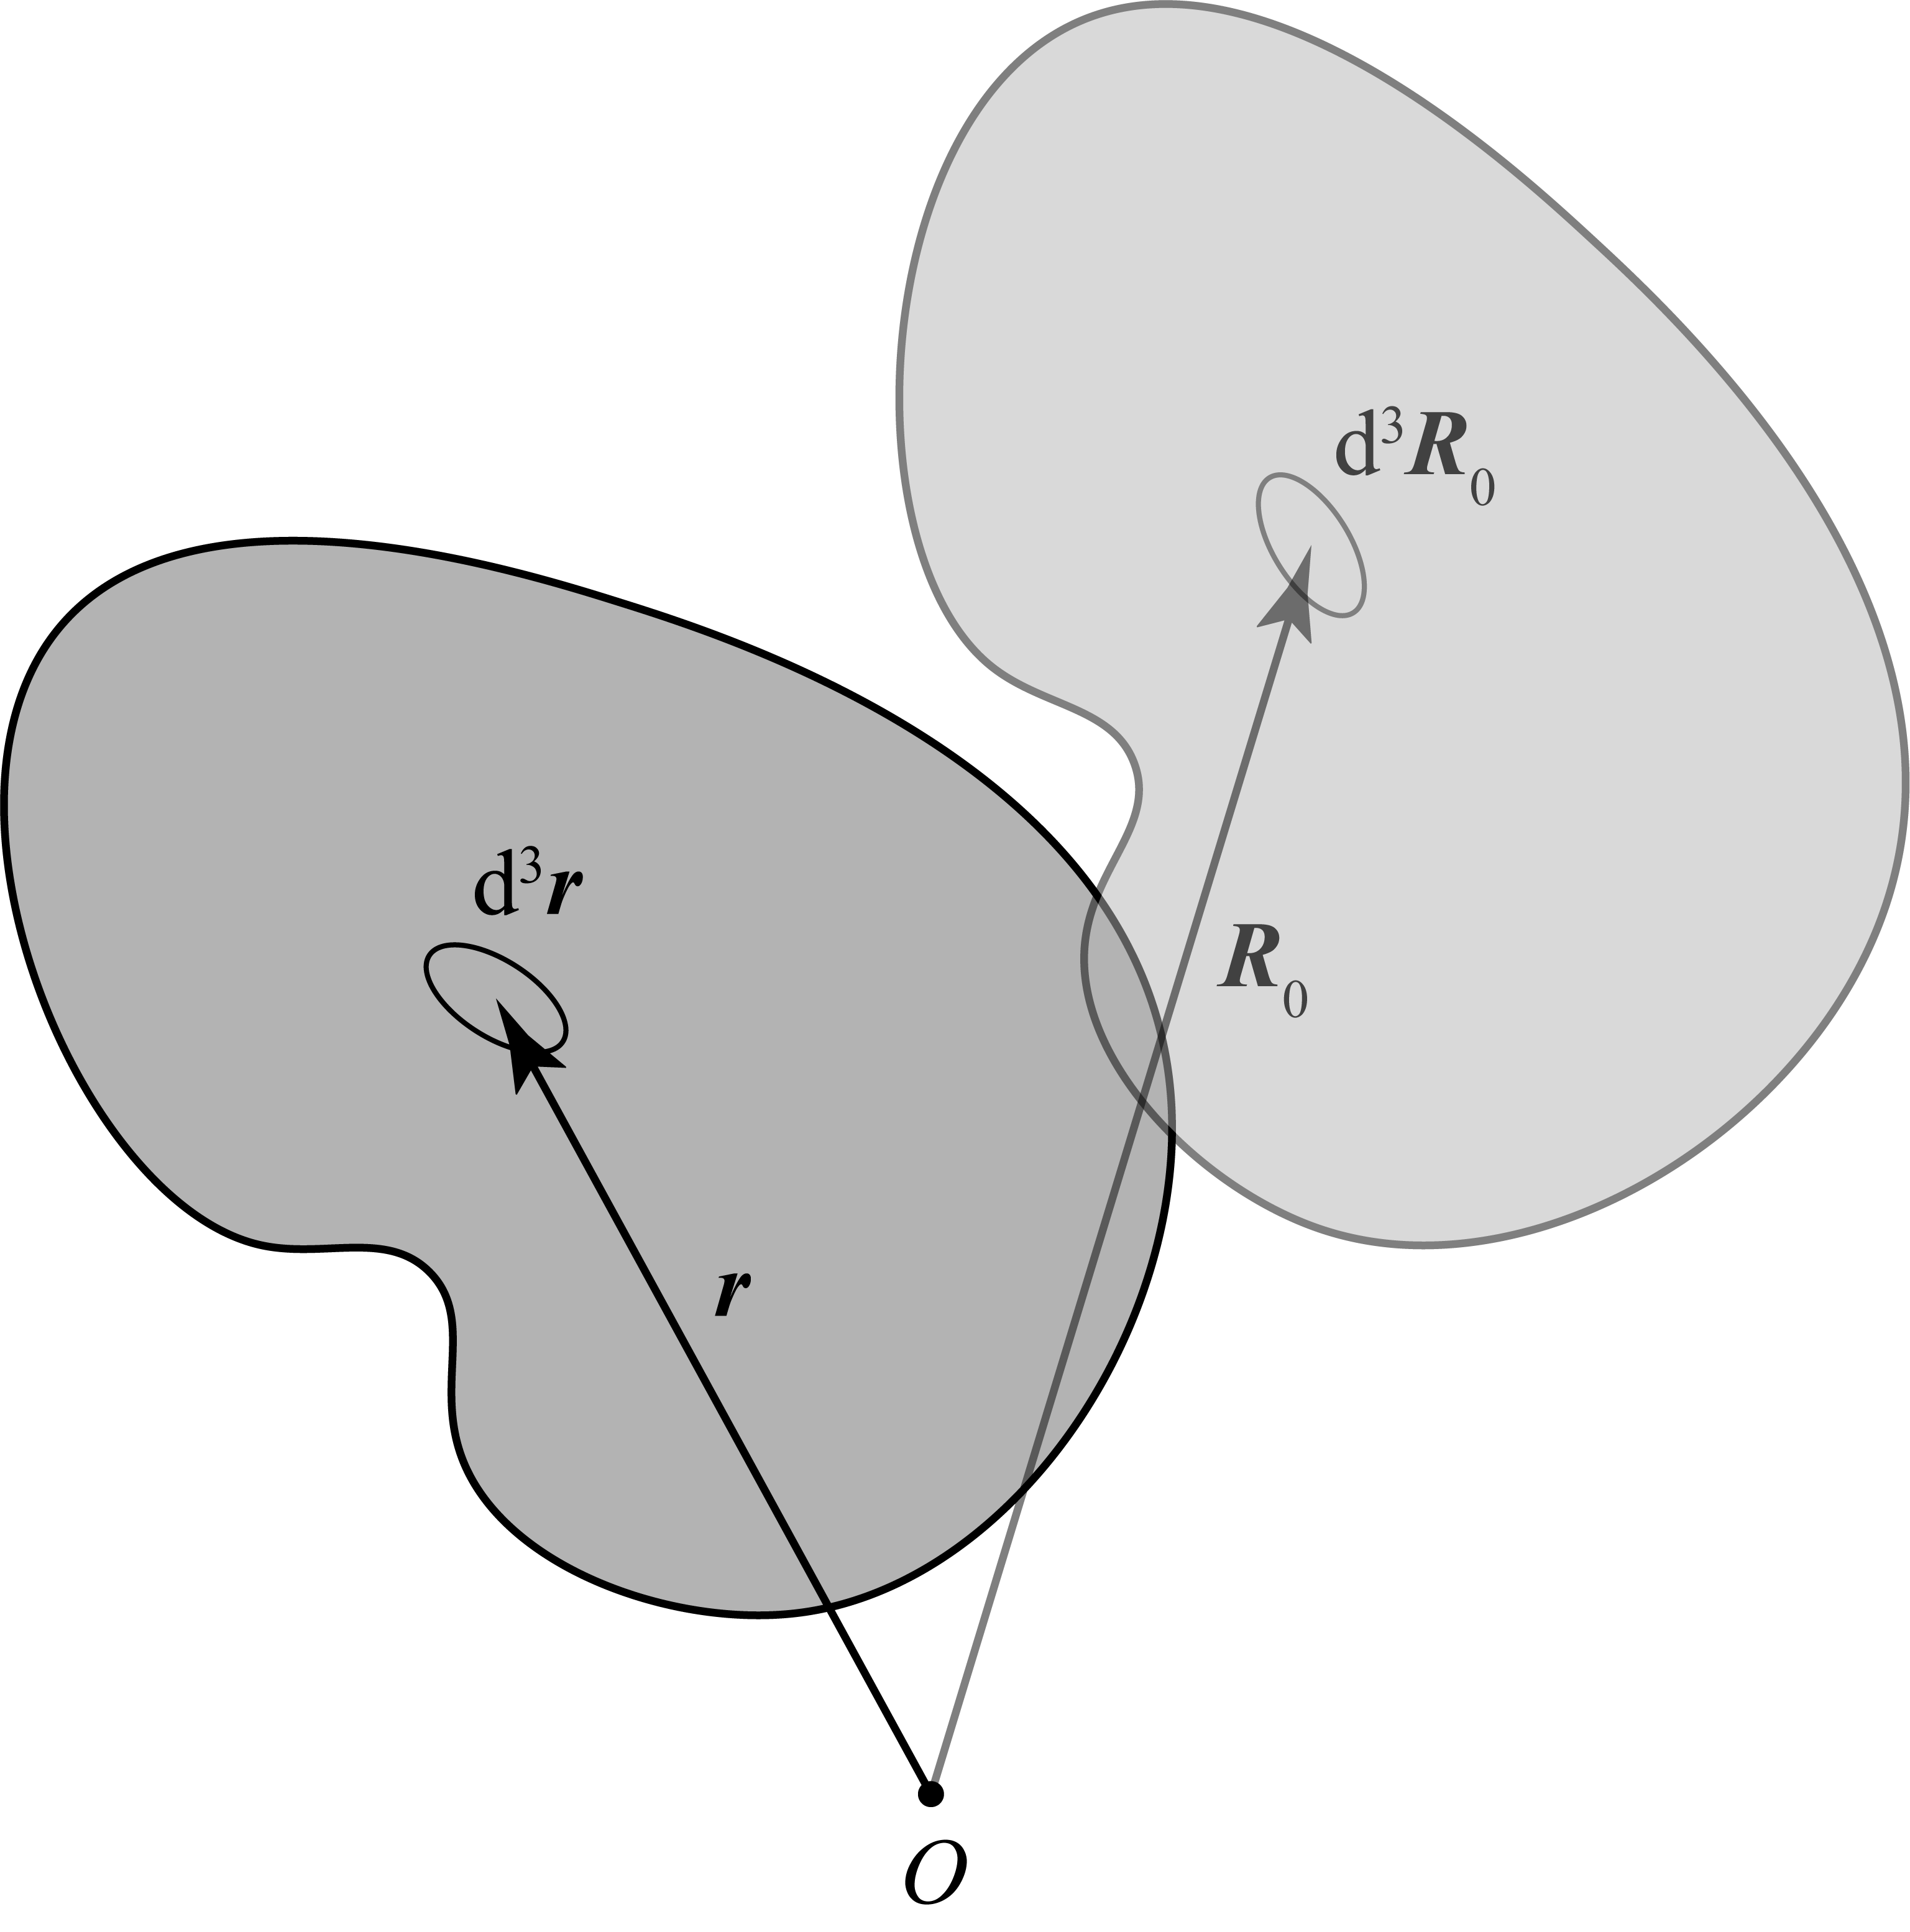
\includegraphics[width=7cm]{image/6-6-1.png}
\caption{刚体的描述}
\end{wrapfigure}
随着刚体的运动,\,原来在$\bs{R}_0$处的体积元现在在$t$时刻位于$\bs{r}$处,\,整个刚体的运动由一个多元映射来定义:
\[f:\quad \bs{R}_0,\,t\;\;\longrightarrow\;\; \bs{r}(\bs{R}_0,\,t)\]

刚体的刚性的要求,\,使得这个映射必须保持体积元的不变性:
\[f:\quad \ud^3\bs{R}_0\in\Omega_0\;\;\longrightarrow\;\; \ud^3\bs{r}\in\Omega \quad ;\quad \ud^3\bs{R}_0=\ud^3\bs{r}=\ud V\]

而且所有这个体积元内的所有内禀属性,\,这里包括密度都不能变.\,所以质量元$\ud m$也是不变的.\,从而刚体具有不变的总质量.\,马上就会发现,\,\emph{质量几何}(mass geometry)对刚体的动力学来说也十分重要.\,质量几何研究质量对特定原点$O$的各级\emph{矩}(moment).\,其中零级矩即为质量:
\[M^0=m=\int\limits_\Omega \ud m\]

一级矩是个矢量,\,它定义了刚体的\emph{质心}(center of mass)的位置:
\[M^1_i=mr_{Ci}=\int\limits_\Omega r_i\ud m\]
\[\bs{r}_C=\frac{\int\limits_\Omega \bs{r}\ud m}{\int\limits_\Omega \ud m}\]

二级矩则是一个张量,\,它的九个分量代表\emph{惯量积}(product of inertia):
\[M^2_{ij}=\int\limits_\Omega r_ir_j\ud m\]

这些矩和原点的选取有关,\,随着刚体的运动也会不断变化,\,这三阶矩的信息对刚体动力学来说就是充分的了,\,通过后面的动力学可以发现,\,刚体的运动完全依赖于外力和这三阶矩.\,如果要研究广义相对论里的引力波辐射问题,\,更高阶的矩才变得重要起来.

刚体的运动可以被我们更精确地描述,\,在$t_0$时刻建立固定在刚体上,\,沿$x,y,z$三方向的单位矢量$\bs{e}_1,\bs{e}_2,\bs{e}_3$,\,那么刚体的运动同时也把三个矢量旋转到新的三个方向:
\[f:\quad \bs{e}_i\;\longrightarrow\; \bs{\varepsilon}_i\]

这三个矢量仍然要互相垂直,\,且长度为一.\,这在数学上导致了可以通过这三个矢量的导数定义\emph{角速度}(angular velocity)矢量的结果:
\[\dot{\bs{\varepsilon}}_i=\bs{\omega}\times\bs{\varepsilon}_i\]

\begin{wrapfigure}[15]{o}[-10pt]{7cm}
\vspace{-0.7cm}
\centering
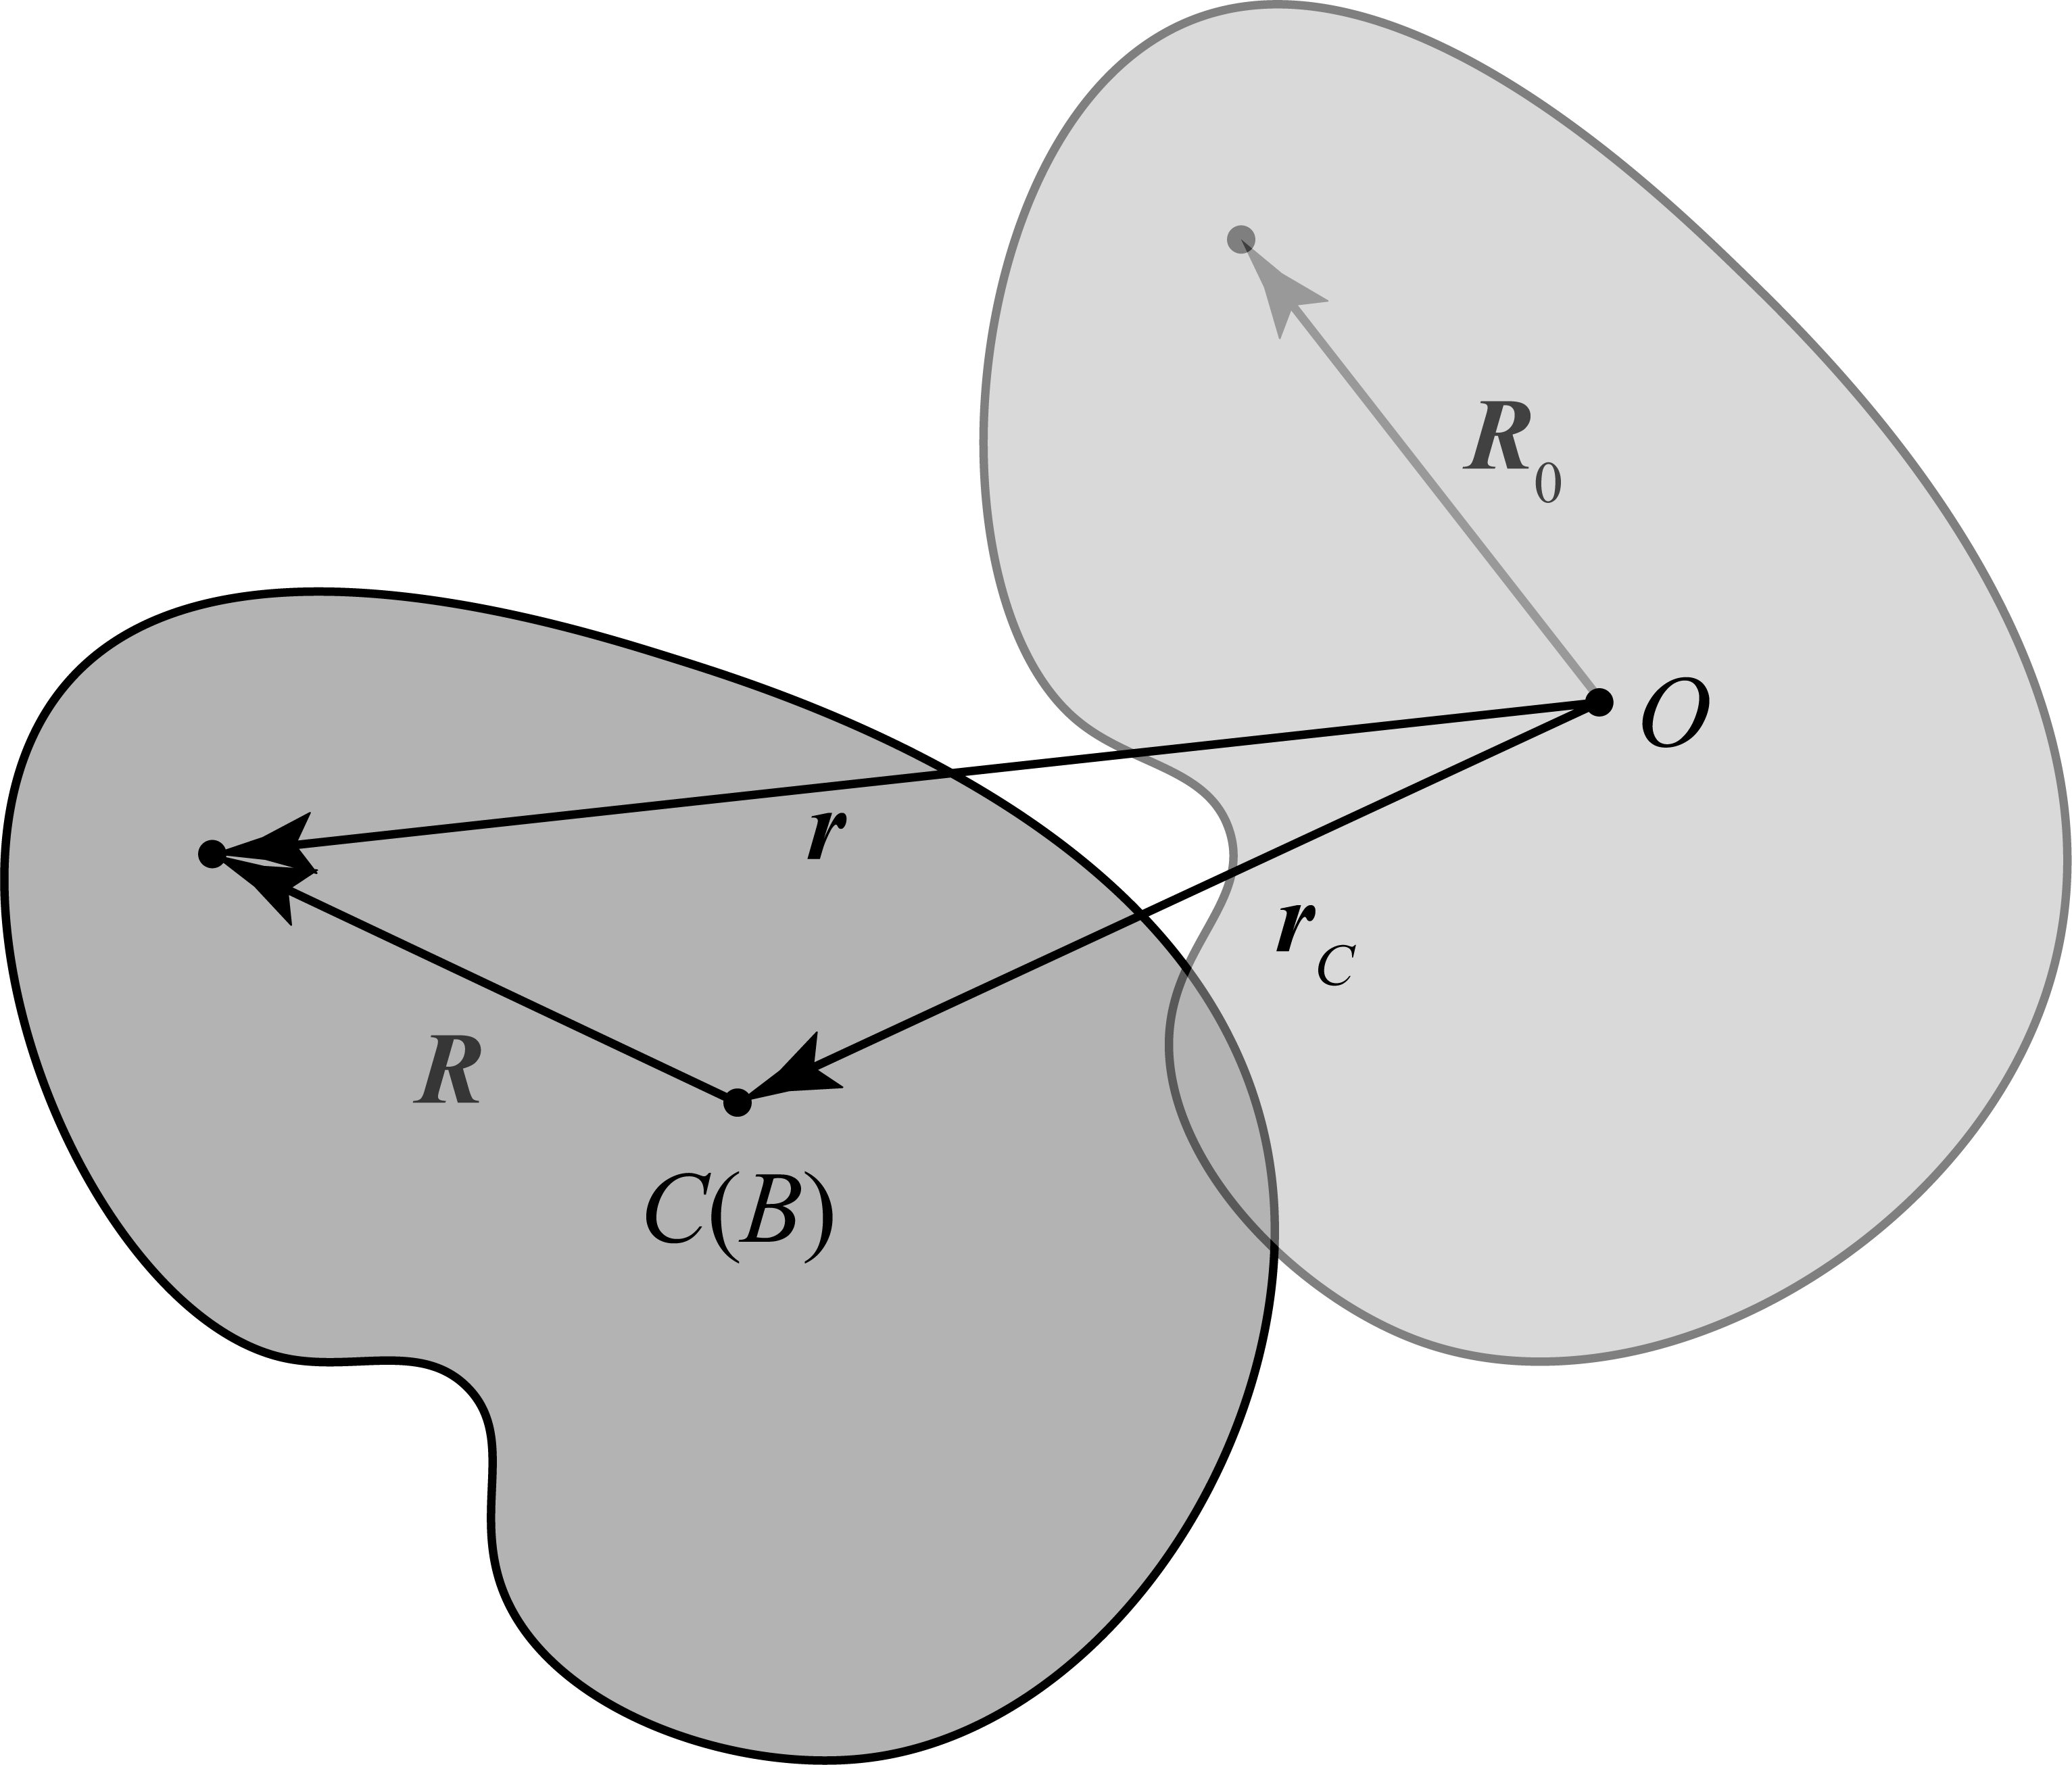
\includegraphics[width=7cm]{image/6-6-2.png}
\caption{基点法}
\end{wrapfigure}
十分类似于旋转参考系的变换的运动学,\,刚体的运动实际上就是有一个唯一的旋转参考系固连在刚体上,\,以后称作\emph{刚体系}(reference system of rigid body),\,要研究的刚体上各个点速度实际上就是刚体系中定点的运动.\,于是习惯上我们采用\emph{基点法}(method of base point)来计算刚体上任意点的运动学量.\,定义\emph{基点}(base point)为$t_0$时刻$\bs{R}_0=\bs{0}$的点$B$,\,之后的位矢为$\bs{r}_B$,\,对应的基点速度加速度为$\bs{v}_B,\,\bs{a}_B$,\,而刚提上待研究的点相对基点的位矢为$\bs{r}-\bs{r}_B=\bs{R}$,\,那么该点的速度加速度即为:
\[\bs{v}=\bs{v}_B+\bs{\omega}\times\bs{R}\]
\[\bs{a}=\bs{a}_B+\bs{\omega}\times(\bs{\omega}\times\bs{R})+\dot{\bs{\omega}}\times\bs{R}\]

出于动力学的考虑,\,基点$B$一般就取做质心$C$.\,作用在刚体上$\bs{r}$处的力$\bs{F}$固然对原点会有力矩$\bs{M}$,\,但是为了研究使刚体自身转动的效应,\,考虑到这个力同时也会使得质心运动起来,\,故我们重视这个力相对质心的力矩$\bs{M}_C$:
\[\bs{M}=\bs{r}\times\bs{F}\]
\[\bs{M}_C=\bs{R}\times\bs{F}\]

刚体受到一个力系${\bs{F}_i}$的作用,\,那么以下六个定理则来自于之前的动力学理论:
\[\sum_i\bs{F}_i=\frac{\ud \bs{p}}{\ud t}\quad ; \quad \sum_i\bs{F}_i=m\bs{a}_C\]
\[\sum_i \bs{v}_i\cdot \bs{F}_i=\frac{\ud }{\ud t}(\frac{1}{2}m\bs{v}_C^2+E_{kr})\quad ;\quad \sum_i(\bs{v}_i-\bs{v}_C)\cdot \bs{F}_i=\frac{\ud E_{kr}}{\ud t}\]
\[\sum_i \bs{r}_i\times \bs{F}_i=\frac{\ud }{\ud t}(\bs{r}_C\times m\bs{v}_C+\bs{L}_r)\quad ;\quad \sum_i \bs{R}_i\times \bs{F}_i=\frac{\ud \bs{L}_r}{\ud t}\]

前两个式子实际上几乎没有区别,\,因为刚体的总动量其实就是质心动量$\bs{p}=m\bs{v}_C$.\,后面几个式子则涉及到相对(平动)质心系的能量与角动量.\,它们与质量二级矩有着密切的联系,\,我们在第三讲\ref{6.3}阐明.\,现在我们写出相对质心系能量角动量的定义:
\[E_{kr}=\int\limits_\Omega \frac{1}{2}(\bs{\omega}\times \bs{R})^2\ud m\]
\[\bs{L}_r=\int\limits_\Omega \bs{R}\times(\bs{\omega}\times \bs{R})\ud m\]




\section{平面平行运动}
一个底面磨平的物体贴在平坦的地面上运动给人以\emph{平面平行运动}(plane-parallel motion)的概念.\,其他的一些物体运动特征也相似于它:\,黑板刷在黑板上的运动,\,车轮在直行时的滚动...\,它们的特征是:\,刚体任何一个体积元都在一个特定的平面上运动,\,而这些平面又彼此平行.\,对于这样的运动基点法只需要给出质心$C$的位矢$\bs{r}_C$和对$t_0$时刻刚体转过的角度$\theta$即可.\,角速度与角加速度即可用角度的导数来给出$\omega=\dot{\theta},\,\beta=\ddot{\theta}$.\,一般来说,\,在垂直于这些平面方向要么由于动力学对称性不需要也不存在任何作用力.\,要么这些力作为约束平面对物体的约束力而不在我们考虑范围内.\,所以我们对一些物理对象做如下修改:\,
\begin{itemize}
\item 所有参考点改成垂直平面过该点的参考轴.\,并约定其正方向
\end{itemize}
\section{空间刚体运动*}\label{6.3}


